\section{Image To Video Model} \label{app:i2v}
We finetune an image-to-video model from the text-to-video model. Drawing from the \citep{blattmann2023stable}, we add an image as an additional condition alongside the text. The image is passed through 3D VAE and concatenated with the noised input in the channel dimension. Similar to super-resolution tasks, there is a significant distribution gap between training and inference (the first frame of videos vs. real-world images). To enhance the model's robustness, we add large noise to the image condition during training. Some examples are shown in Figure~\ref{fig:i2vgood1}, Figure~\ref{fig:i2vgood2}. CogVideoX can handle different styles of image input.

\begin{figure}[ht]
\begin{center}
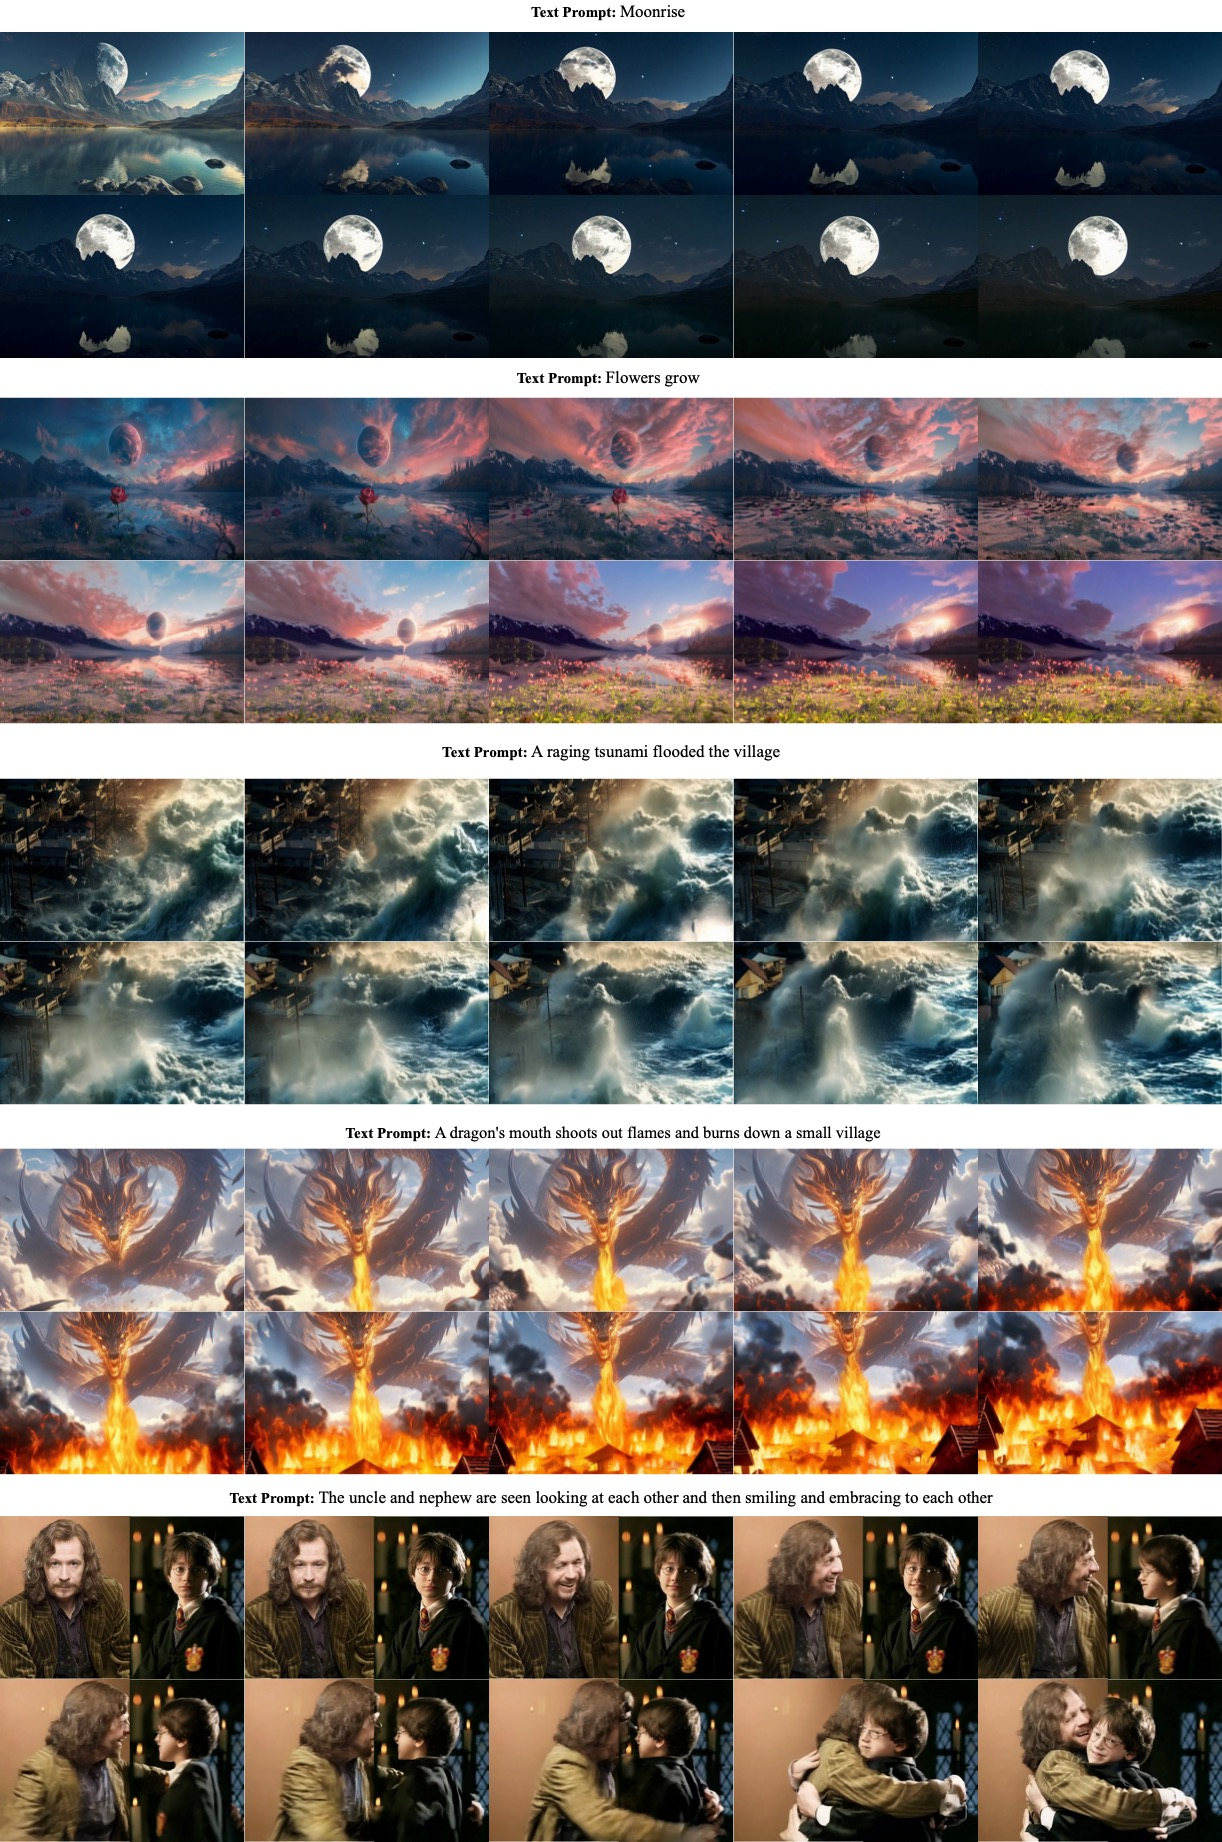
\includegraphics[width=\linewidth]{images/t2v/i2vgood1.jpg}
\end{center}
\caption{Image to video showcases. The displayed prompt will be upsampled before being fed into the model.}
\label{fig:i2vgood1}
\end{figure}

\begin{figure}[ht]
\begin{center}
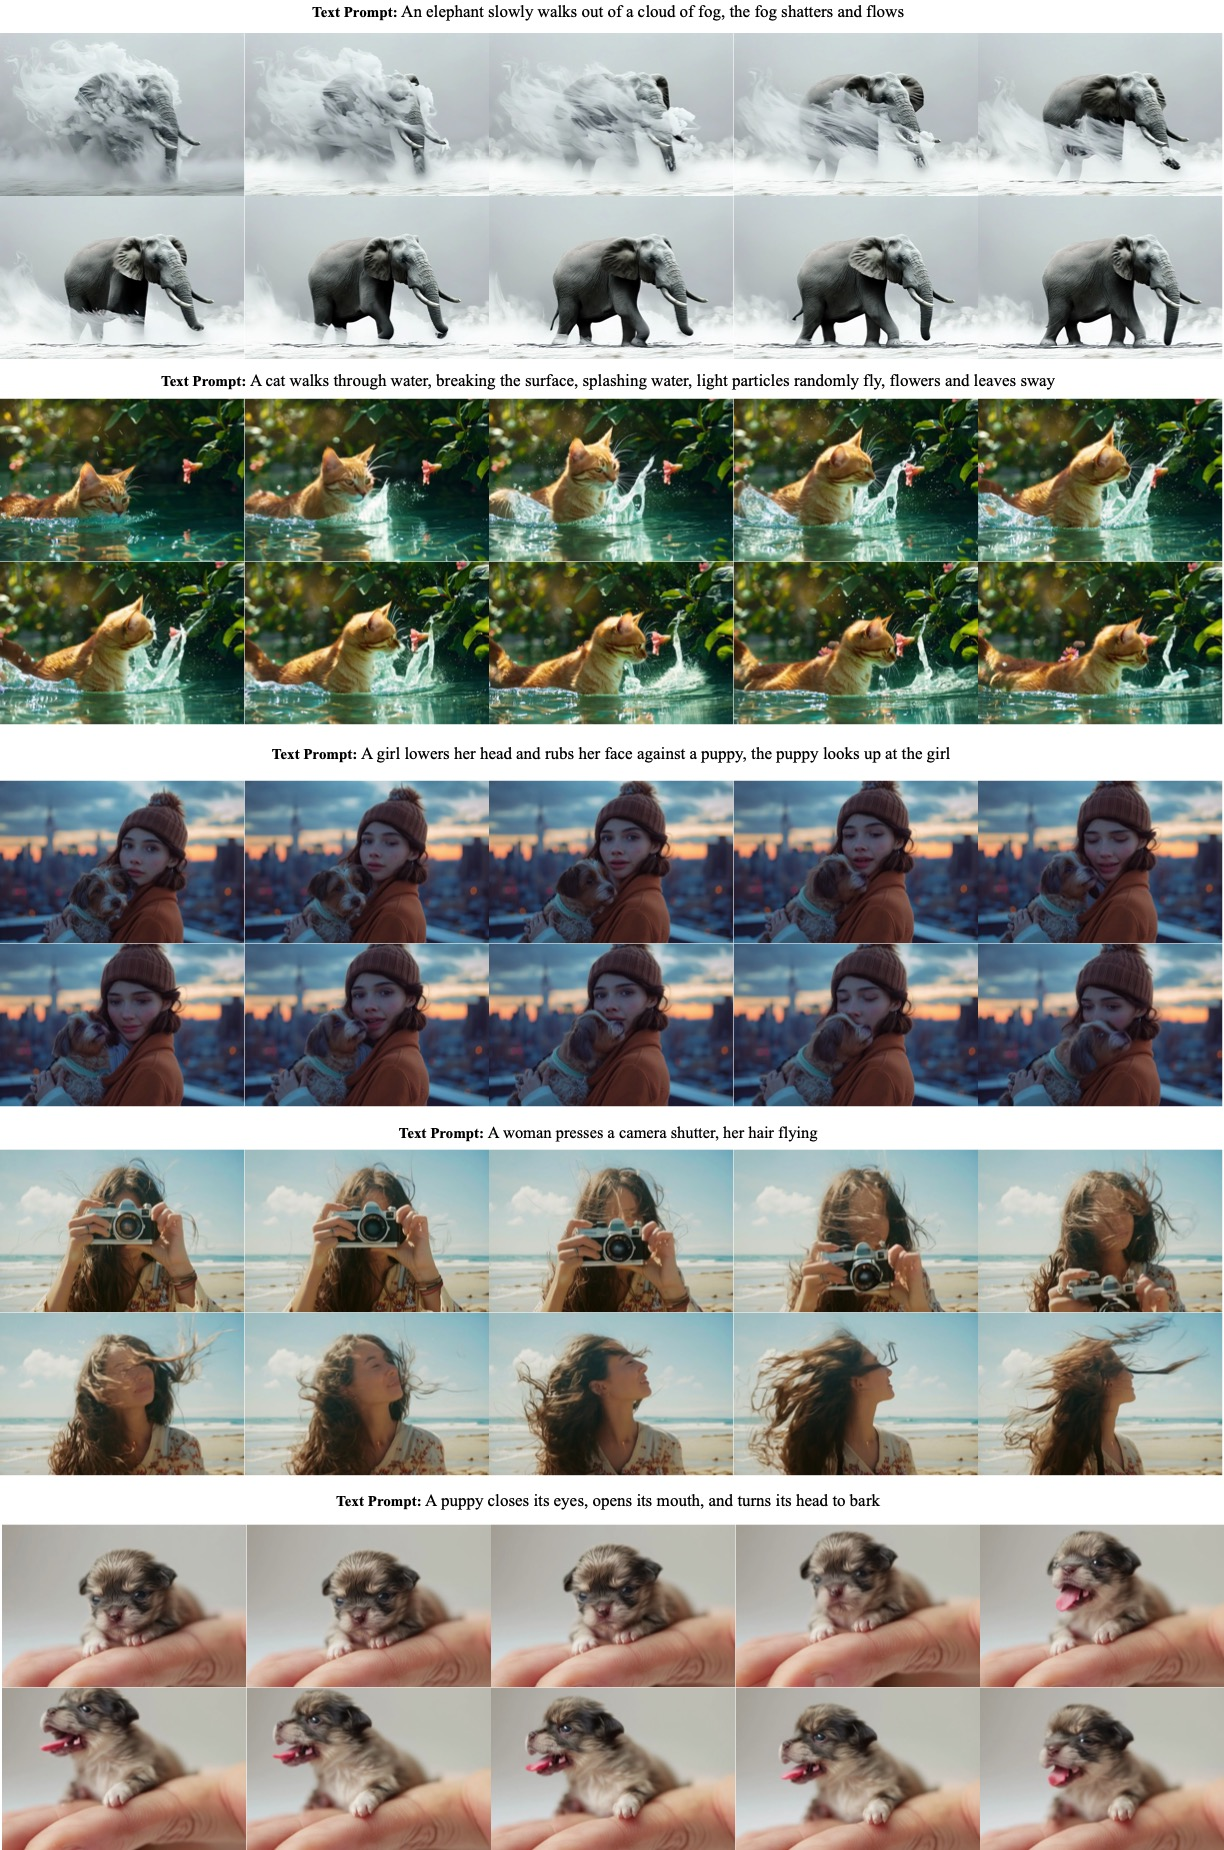
\includegraphics[width=\linewidth]{images/t2v/i2vgood2.jpg}
\end{center}
\caption{Image to video showcases.}
\label{fig:i2vgood2}
\end{figure}